% additional_parts.tex
% used to read parts to main.tex tiedostoon
% see: https://texblog.org/2012/12/04/keeping-things-organized-in-large-documents/
% loading part that are sepated with their tags 
% starting and ending with %<*tagname> and  %</eq:tagname>

%%%%% Equations
%<*eq:contpid>
\begin{equation} \label{eq:contpid}
	u(t)=K_pe(t) + K_i\int_{0}^{t} e(\tau) d\tau + K_d\frac{de(t)}{dt}
\end{equation}
%</eq:contpid>

%%%%% Tables
%<*table:messivsronaldo>
\begin{table}[htb]\footnotesize 
	\caption{Club goals for Messi and Ronaldo between seasons 2017-2018 and 2019-2020.}
	\centering
	\begin{tabular}{@{}lrrr@{}}
		\hline % \toprule
		Player & 2017-2018 & 2018-2019 & 2019-2020 \\ 
		\hline %\midrule
		Messi & 45 & 51 & 31 \\
		Ronaldo & 44 & 28 & 37 \\
		\hline % \bottomrule
	\end{tabular}
	\label{table:messivsronaldo}
\end{table}
%</table:messivsronaldo>

%%%% Figures
%<*fig:sine>
\begin{figure}[htb]
	\centering
	% 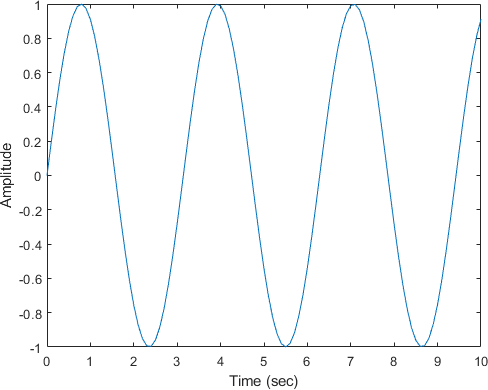
\includegraphics[width=1\textwidth]{./figs/fig_sine.png}
	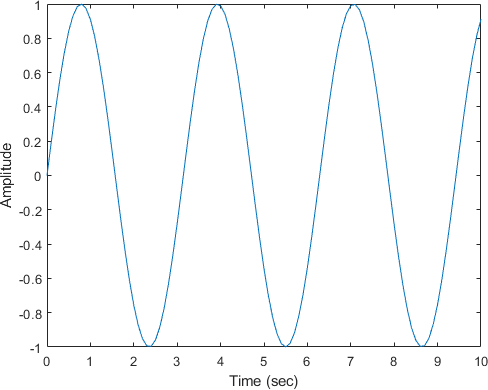
\includegraphics[width=0.25\textwidth]{./figs/fig_sine.png}
	\caption{Sine signal. \label{fig:sine}}
\end{figure}
\FloatBarrier
%</fig:sine>

%<*fig:closedloop>
\begin{figure}[htb]
	\centering
	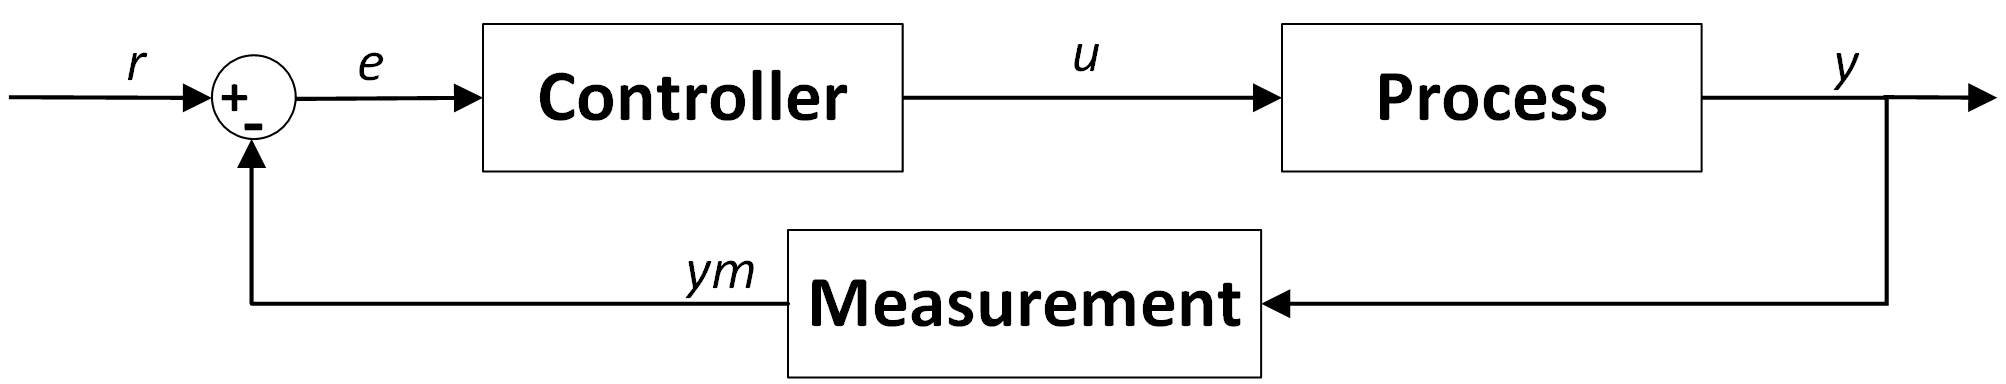
\includegraphics[width=1\textwidth]{./figs/closed_loop.png}
	\caption{second fig. \label{fig:closedloop}}
\end{figure}
\FloatBarrier
%</fig:closedloop>




